\documentclass[11pt]{article}

\usepackage[margin=1in]{geometry}
\usepackage{amsmath,amssymb,amsthm}
\usepackage{booktabs}
\usepackage{graphicx}
\usepackage{hyperref}
\usepackage{xcolor}
\usepackage{listings}
\usepackage[numbers,sort&compress]{natbib}
\usepackage{authblk}
\usepackage{enumitem}

\hypersetup{
    colorlinks=true,
    linkcolor=blue,
    urlcolor=blue,
    citecolor=blue,
}

\title{Composable KV:\\ Position Alignment and Lightweight Value Correction\\ for Independent LLM Prefill Cache Composition}

\author[1]{Mun Yunhyuk\thanks{\texttt{moonyoonh91@gmail.com}}}
\affil[1]{Independent research}

\date{\today}

\begin{document}
\maketitle

\begin{abstract}
Large language model serving increasingly relies on caching independent prefix key--value (KV) representations for reuse across queries. Composing two independently prefilled caches, however, yields degraded next-token behavior compared to a full joint prefill. We conceptually separate this degradation into two error sources -- a \emph{position mismatch} (rotary encoding assumes each token's absolute index) and a \emph{cross-context representation mismatch} (each cache never attended to the other), and study the two error sources separately on Qwen-2.5-0.5B. Positional alignment via RoPE-shift improves top-1 agreement with the full-prefill baseline in three of four controlled conditions but does not uniformly reduce Kullback--Leibler divergence to the oracle, demonstrating that the two behavioral metrics can diverge. A layer-selective RoPE-shift (skipping mid layers where the per-layer value cosine drops most) yields no improvement over full RoPE-shift, indicating that layer selection alone does not close the mid-layer gap. We introduce a single $64\times64$ linear map applied to the middle-layer value cache, trained by ridge-regularized least squares to predict the full-prefill value from the independent value. Across four cross-validated folds at the example level of a $20$-example controlled benchmark, the corrector reduces held-out downstream next-token KL by 6.4\% on naive concatenation and 9.4\% on RoPE-shifted concatenation, and reduces KL on each of the four conditions; in-sample and held-out KL agree within $3\times10^{-3}$, suggesting that the corrector transfers to held-out examples within this benchmark rather than fitting to specific training instances. The correction adds approximately $0.34$ ms of wall-clock and $\sim 0.0021\%$ of the FLOPs of one full $B$-prefill. Its singular-value spectrum is nearly full-rank ($\lVert W - I \rVert_F / \lVert W \rVert_F = 0.76$), and rank truncations below $k \approx 22$ underperform the un-corrected baseline, indicating the correction is distributed across many $V$ dimensions rather than concentrated in a small subspace. All numbers are supported by a set of pipeline sanity checks (cache round-trip KL $\approx 3\times10^{-7}$, RoPE-shift-by-zero is exact identity, prefill is deterministic, and the $A$-portion of the joint cache matches the standalone $A$ prefill within float32 precision). We frame this as a proof of feasibility on a small controlled benchmark, with concrete follow-ups toward scale, model families, and realistic serving workloads.
\end{abstract}

\section{Introduction}

Autoregressive language model inference under long context is dominated by the KV cache: for every generated token, the model attends to all previous keys and values, whose memory footprint scales linearly with context length. Serving systems accordingly cache and share prefix KVs~\citep{kwon2023vllm,zheng2024sglang,gim2023prompt}. In an idealized reuse pattern, one would prefill an arbitrary prefix $A$, prefill an arbitrary prefix $B$ independently, and combine them at query time without paying the cost of jointly reprocessing $A+B$.

The behavior of such an independent-prefill composition, however, differs from the behavior of a joint prefill in ways that matter. Two error sources are structurally distinct:

\begin{enumerate}[leftmargin=*]
    \item \textbf{Position mismatch.} Rotary Positional Embedding (RoPE)~\citep{su2021roformer} applies a position-dependent rotation to each key. A key that was originally at position $p_B$ in $B$-alone remains at rotation angle $p_B \cdot \theta_i$; if we place it at absolute position $|A| + p_B$ in the composed cache, the query at the new position attends against a key whose rotation encodes the wrong offset.
    \item \textbf{Cross-context representation mismatch.} During a joint prefill, each layer's hidden state for tokens in $B$ is computed after attending to tokens in $A$. The $B$-tokens' keys and values consequently \emph{depend on the specific content of $A$}. When $B$ is prefilled in isolation, no such attention has ever occurred, and no positional operation on the isolated cache can recover the missing content-dependent interaction.
\end{enumerate}

Position mismatch is fixable in principle by shifting each stored $B$-key back to its intended composed position. Cross-context mismatch is not: it is a fact about the counterfactual computation that was never performed. Any attempt to close it must inject an approximation of the missing $A$-conditional information into the cached representation directly.

This paper asks: \emph{on a small controlled benchmark, does a low-cost learned correction of the middle-layer value cache partially close the cross-context error, and does that improvement survive an example-level held-out split?}

\paragraph{Contributions.}
\begin{itemize}[leftmargin=*]
    \item We articulate two conceptually distinct error sources (position mismatch and cross-context representation mismatch) and design four controlled conditions (independent, referential, conflicting, cross-inferential) that vary the degree to which $B$ semantically depends on $A$.
    \item We provide layer-wise per-head analysis of both key and value divergence between independent-prefill $B$ and joint-prefill $B$, showing a mid-layer dip in value cosine that is consistent with the general observation that middle layers perform semantic integration.
    \item We test whether layer selection alone can route around the mid-layer damage (Method M3) and find no improvement over full RoPE-shift, motivating a learned intervention.
    \item We introduce a single $64\times64$ linear map on the layer-12 value cache and show, on a 5-fold example-level held-out split of a 20-example benchmark, that it reduces downstream next-token KL by 6.4--9.4\% relative to un-corrected baselines, and reduces KL on each of the four conditions in this benchmark. In-sample and held-out KL agree within $3\times10^{-3}$, suggesting transfer to held-out examples within this benchmark (rather than a stronger claim of generalization, which would require entity- or template-disjoint splits).
    \item We quantify wall-clock and FLOP cost, showing the corrector is approximately $0.0021\%$ of a single $B$-prefill in FLOPs, and validate the cache-injection pipeline against a $\sim 3\times10^{-7}$ KL noise floor.
    \item We are explicit about what these results \emph{do not} yet show: single model (0.5B), single family (Qwen), $n=20$ controlled examples, no realistic serving workload, no MLP or multi-layer corrector.
\end{itemize}

\section{Related Work}

\paragraph{KV cache compression and eviction.} A large body of recent work reduces the memory footprint of the KV cache by dropping, quantizing, or pooling entries: H2O~\citep{zhang2023h2o}, StreamingLLM~\citep{xiao2023streamingllm}, SnapKV~\citep{li2024snapkv}, DuoAttention~\citep{xiao2024duoattention}. These operate on a single already-computed cache and preserve or approximate its content; they do not compose independently computed caches.

\paragraph{Prefix caching in serving systems.} vLLM's automatic prefix cache~\citep{kwon2023vllm}, RadixAttention in SGLang~\citep{zheng2024sglang}, and Prompt Cache~\citep{gim2023prompt} share exact-match prefixes at query time. When multiple requests share a literal prefix, the prefix is prefilled once and reused. Our setting is complementary: we ask whether \emph{non-shared} prefixes computed independently can be combined at all, not whether an exact-match prefix can be reused.

\paragraph{Representation arithmetic.} Task Arithmetic~\citep{ilharco2022editing} composes weight-space fine-tune deltas by addition. Activation steering~\citep{turner2023activation} adds direction vectors to hidden states. We instead operate on cached keys and values at inference time, but share the family perspective: learned linear operations on internal representations can produce nontrivial behavioral changes.

\paragraph{YOCO and cache reuse.} YOCO~\citep{sun2024yoco} restructures the decoder so a single cache is shared across half the layers. This is architectural rather than a run-time composition of independent caches, but it points at the same underlying goal of reducing redundant prefill.

\paragraph{Long-context and cross-attention.} A rich literature investigates how information from earlier positions is integrated at each layer~\citep{elhage2022superposition,olah2022attention}. The mid-layer semantic integration observation we rely on is consistent with these interpretability findings.

\section{Problem Formulation}

Given a decoder-only Transformer with $L$ layers, $H$ key-value heads, and head dimension $d$, let $\mathrm{prefill}(X)$ denote the cache produced by processing token sequence $X$. Concretely,
\[
\mathrm{prefill}(X) = \bigl( K^{(l)}(X), V^{(l)}(X) \bigr)_{l=1}^L,
\qquad
K^{(l)}(X), V^{(l)}(X) \in \mathbb{R}^{H \times |X| \times d}.
\]
Given two prefixes $A$ and $B$ with token lengths $|A|$ and $|B|$, the \emph{joint} (oracle) cache is
$\mathrm{KV}_{\text{full}} = \mathrm{prefill}([A;B])$. The \emph{independent} caches are $\mathrm{KV}_A = \mathrm{prefill}(A)$ and $\mathrm{KV}_B = \mathrm{prefill}(B)$. A composition method $\mathcal{C}$ produces a candidate cache
\[
\mathrm{KV}_{\text{comp}}^{\mathcal{C}} = \mathcal{C}\bigl( \mathrm{KV}_A, \mathrm{KV}_B \bigr),
\]
which is then used as the past for a shared query $Q$ to produce a next-token distribution $p_{\text{comp}}^{\mathcal{C}}$. The oracle distribution $p_{\text{full}}$ is produced by $\mathrm{prefill}([A;B;Q])$.

We measure composition quality on two behavioral metrics:
\[
\mathrm{KL}(p_{\text{full}} \Vert p_{\text{comp}}^{\mathcal{C}}),
\qquad
\mathrm{Agree@}k(p_{\text{full}}, p_{\text{comp}}^{\mathcal{C}})
= \frac{|\mathrm{top}_k(p_{\text{full}}) \cap \mathrm{top}_k(p_{\text{comp}}^{\mathcal{C}})|}{k}.
\]

We use $k \in \{1, 5, 10\}$. As we show in Section~\ref{sec:m2}, these two metrics can move in opposite directions.

\subsection{Methods}

\paragraph{M1: Naive concatenation.} $K^{(l)}$ and $V^{(l)}$ are simply concatenated along the sequence dimension:
\[
K^{(l)}_{\text{comp}} = [K^{(l)}_A ; K^{(l)}_B],
\quad
V^{(l)}_{\text{comp}} = [V^{(l)}_A ; V^{(l)}_B].
\]
This ignores position, and $K^{(l)}_B$ retains RoPE rotations for positions $0, \dots, |B|-1$ even though it will be used as if it sits at positions $|A|, \dots, |A|+|B|-1$.

\paragraph{M2: RoPE-shifted concatenation.} Because RoPE is applied to $K$ prior to caching, and because rotations in a single frequency band commute, applying an additional rotation by $|A|$ produces the same $K$ we would have stored had $B$ been at positions $|A|, \dots, |A|+|B|-1$ from the outset (assuming the same underlying hidden state, which of course is not the case; see Section~\ref{sec:m2}):
\[
K^{(l)}_{\text{shifted}, i} = R\bigl( |A| \cdot \theta \bigr) \cdot K^{(l)}_{B, i}
\quad \forall i,
\]
where $R(\phi)$ denotes the standard half-rotation RoPE rotation by angle $\phi$. $V$ is unchanged. On our test example (independent \#0, $|A|=16$, $|B|=19$), the layer-averaged $K$ cosine between $B$-alone shifted and $B$-in-full grows from $0.817$ (raw) to $0.923$ (shifted), and layer L0 achieves cosine $1.0000$, verifying the implementation.

\paragraph{M3: Layer-selective RoPE-shift.} Since layer-wise analysis (Section~\ref{sec:layers}) shows a mid-layer dip in value cosine, one might hypothesize that RoPE-shift damages the mid layers by imposing a false alignment there. M3 applies RoPE-shift to all layers \emph{except} $\{L_{10}, \ldots, L_{15}\}$.

\paragraph{H3: Learned value corrector.} At a target layer $l^\star$ (we use $l^\star = 12$), we replace $V^{(l^\star)}_B$ with $\hat V^{(l^\star)}_B = V^{(l^\star)}_B W$, where $W \in \mathbb{R}^{d \times d}$ is fit by ridge-regularized least squares on training examples' $(V^{(l^\star)}_B, V^{(l^\star)}_{B|A})$ pairs. We compose M4 = M1 + H3 and M5 = M2 + H3.

\section{Experimental Setup}

\paragraph{Model.} All experiments use \texttt{Qwen/Qwen2.5-0.5B}~\citep{qwen2025qwen25}. Architecture: 24 layers, 14 query heads, 2 KV heads (grouped-query attention), head dimension 64, hidden size 896, RoPE base $\theta = 10^6$.

\paragraph{Controlled benchmark.} We construct 20 examples spanning four conditions ($n=5$ per condition):
\begin{itemize}[leftmargin=*]
    \item \textbf{independent}: $A$ and $B$ describe unrelated entities; the query concerns only $A$.
    \item \textbf{referential}: $B$ makes a pronominal or nominal reference to an entity introduced in $A$.
    \item \textbf{conflicting}: $A$ and $B$ ascribe contradictory attributes to the same named entity.
    \item \textbf{cross-inferential}: the query's answer requires combining a rule from $A$ with an instance from $B$.
\end{itemize}
The conditions increase in the strength of the cross-context dependency of $B$ on $A$. Full templates are in the released \texttt{conditions.py}.

\paragraph{Sanity checks.} Before running any composition experiments, we verify the pipeline (see Appendix~\ref{app:sanity} for details): cache round-trip KL is $\approx 3\times10^{-7}$; RoPE-shift by 0 is exact identity ($< 10^{-10}$); prefill is deterministic ($0$); the $A$-portion of the joint cache matches the $A$-alone cache within float32 precision ($1.5\times10^{-5}$).

\section{Results}

\subsection{Layer-wise divergence}\label{sec:layers}

For each example we compute per-layer cosine similarity between $\mathrm{KV}_B$ and the $B$-portion of $\mathrm{KV}_{\text{full}}$. Since $V$ has no RoPE rotation, $V$-cosine isolates pure cross-context effect; $K$-cosine mixes cross-context with position offset.

Averaged across the four conditions, $V$-cosine starts near $1.0$ at layer L0, dips to $0.56$--$0.79$ across layers L10--L15 (the greatest dip in the \emph{conflicting} condition at L12), and partially recovers at layers L20--L23. $K$-cosine also drops in the mid layers but recovers less sharply. This mid-layer dip is consistent with prior interpretability work identifying middle layers as loci of semantic integration~\citep{elhage2022superposition}.

\subsection{Method comparison}\label{sec:m2}

Table~\ref{tab:main} reports per-method aggregate KL and top-1 agreement across all 20 examples. Two observations dominate.

\begin{table}[t]
\centering
\caption{Aggregate downstream metrics on the 20-example controlled benchmark, Qwen-2.5-0.5B. \textbf{KL} is Kullback--Leibler divergence from the full-prefill oracle; \textbf{top-$k$} is next-token agreement. Held-out is a 5-fold example-level split. Lower KL is better.}
\label{tab:main}
\begin{tabular}{lrrrrr}
\toprule
Method & KL mean & KL std & top-1 & top-5 & top-10 \\
\midrule
M1 (naive)              & 0.329 & 0.127 & 0.25 & 0.77 & 0.72 \\
M2 (RoPE-shift)          & 0.405 & 0.207 & 0.50 & 0.72 & 0.70 \\
M3 (RoPE-shift ex mid)   & 0.404 & 0.196 & 0.50 & 0.75 & 0.71 \\
M4 (naive + H3)          & \textbf{0.308} & 0.118 & 0.30 & \textbf{0.79} & 0.74 \\
M5 (RoPE-shift + H3)     & 0.367 & 0.196 & \textbf{0.55} & 0.75 & 0.70 \\
\bottomrule
\end{tabular}
\end{table}

\paragraph{Top-1 and KL can diverge.} M2 improves top-1 over M1 in every condition except referential (a tie) but \emph{worsens} KL in independent, referential, and cross-inferential, improving KL only in the \emph{conflicting} condition. Reading M2 as ``conditionally better'' therefore requires committing to a single metric. Reporting both is necessary.

\paragraph{Layer selection alone does not close the mid-layer gap.} M3 differs from M2 only at layers L10--L15, and yet the aggregate difference is within one standard deviation for every condition. The mid-layer value dip is at most a symptom, not an intervention target that layer selection alone can address.

\subsection{Held-out transfer of H3 within the benchmark}\label{sec:holdout}

We train $W \in \mathbb{R}^{64\times64}$ by ridge-regularized least squares (ridge $10^{-4}$) on the layer-12 value pairs across the training portion of a 5-fold example-level split, holding out four examples per fold. Table~\ref{tab:holdout} reports held-out mean KL for each of the four conditions.

\begin{table}[t]
\centering
\caption{Held-out (5-fold, example-level) mean KL per condition. H3 correction reduces KL in every condition when combined with either M1 (naive concat) or M2 (RoPE-shift).}
\label{tab:holdout}
\begin{tabular}{lrrrr}
\toprule
Condition & M1 (naive) & M4 = M1+H3 & M2 (rope) & M5 = M2+H3 \\
\midrule
independent        & 0.338 & 0.329 & 0.441 & 0.415 \\
referential        & 0.295 & 0.293 & 0.511 & 0.466 \\
conflicting        & 0.353 & 0.311 & 0.270 & \textbf{0.228} \\
cross-inferential  & 0.330 & 0.299 & 0.399 & 0.361 \\
\midrule
Aggregate          & 0.329 & \textbf{0.308} & 0.405 & \textbf{0.367} \\
$\Delta$ vs base   &       & $-6.4\%$ &       & $-9.4\%$ \\
\bottomrule
\end{tabular}
\end{table}

The held-out corrector matches its in-sample counterpart within $3\times10^{-3}$ KL, indicating that the improvement transfers to held-out examples within this benchmark (stronger claims of generalization would require entity- or template-disjoint splits, deferred to future work). On the conflicting condition, M5 achieves top-1 agreement $1.00$ on held-out (every held-out example's composed distribution places the same token first as the full-prefill oracle).

\subsection{What does the learned $W$ do?}\label{sec:interp}

To gain intuition for the correction, we compute the singular value decomposition (SVD) of the trained $W$ at layer 12. Figure~\ref{fig:wspec} (left) shows the singular-value spectrum: contrary to a natural first hypothesis, $W$ is not low-rank. Its singular values decay gradually from $\sigma_0 = 1.63$ to a floor of $\sigma_{63} = 0.006$, with 63 of 64 dimensions above $1\%$ of the largest singular value. The Frobenius distance from the identity, $\lVert W - I \rVert_F / \lVert W \rVert_F = 0.76$, confirms that $W$ is not close to a pass-through.

Figure~\ref{fig:wspec} (right) reports mean cosine similarity of $V_B W_k$ against $V_{B \mid A}$, where $W_k$ is the rank-$k$ truncation of $W$. Two observations stand out:

\begin{itemize}[leftmargin=*]
    \item \textbf{Low-rank truncations underperform the un-corrected baseline.} A rank-1 $W$ degrades cosine to $0.13$; the corrected cosine only exceeds the un-corrected $0.616$ at $k \approx 22$.
    \item \textbf{Correction gain accumulates over most of the spectrum.} Rank-48 $W$ ($75\%$ of the spectrum) recovers $90\%$ of the full-rank gain; rank-24 recovers only $11\%$.
\end{itemize}

The cross-context correction at this layer is therefore not concentrated in a small subspace. Naive rank compression of the corrector is not viable, and non-linear alternatives (MLP, $A$-context-conditional) will still need enough capacity to route information through many dimensions of $V$ rather than isolate a few dominant modes.

\begin{figure}[t]
\centering
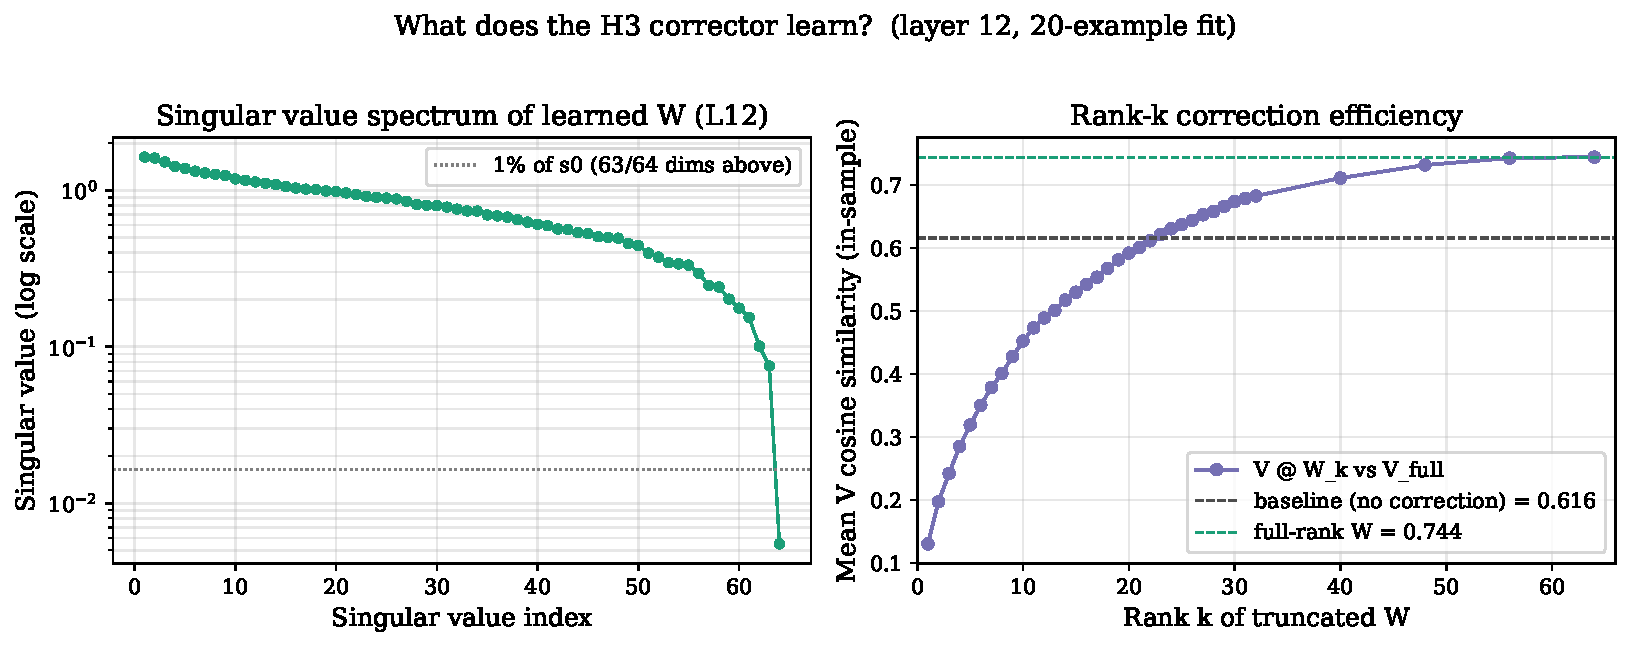
\includegraphics[width=\textwidth]{W_spectrum.pdf}
\caption{Left: singular values of the trained $64\times64$ corrector $W$ (log scale); the spectrum is nearly full-rank. Right: rank-$k$ truncated $W_k$ evaluated in-sample by mean $V$ cosine similarity. Gain relative to the un-corrected baseline (grey dashed) becomes positive only around $k \approx 22$, and reaches $90\%$ of the full-rank gain (green dashed) at $k = 48$.}
\label{fig:wspec}
\end{figure}

\subsection{Cost}\label{sec:cost}

Wall-clock measurements on CPU (median of five runs, $|B|=19$) are reported in Table~\ref{tab:cost}. Composition itself (M1, M2) is under $5\%$ of one $B$-prefill. The H3 correction adds approximately $0.34$ ms and $\sim 311{,}000$ FLOPs (a $64\times64$ matmul on $|B|\cdot H_{\mathrm{kv}} = 38$ rows), i.e.\ $\sim 0.0021\%$ of the estimated $\sim 14.85$ GFLOPs required for one $B$-prefill forward.

\begin{table}[t]
\centering
\caption{Wall-clock cost of composition on CPU, relative to a single $B$-prefill forward. Setup: Qwen-2.5-0.5B, CPU (single-thread PyTorch), $|B|=19$ tokens, $\mathrm{KV}_A$ and $\mathrm{KV}_B$ already computed and in memory (KV storage / transfer costs are not measured). H3 correction is a $64\times64$ matmul at a single layer. Numbers are the median of 5 runs.}
\label{tab:cost}
\begin{tabular}{lrr}
\toprule
Operation & Wall-clock (ms) & \% of prefill($B$) \\
\midrule
prefill($B$) baseline           & 344.9 & 100.00 \\
M1 naive concat                 &   3.1 &   0.91 \\
M2 RoPE-shift concat            &  14.1 &   4.08 \\
M4 naive + H3 correction        &   3.5 &   1.00 \\
M5 RoPE-shift + H3 correction   &  13.4 &   3.90 \\
\bottomrule
\end{tabular}
\end{table}

\begin{figure}[t]
\centering
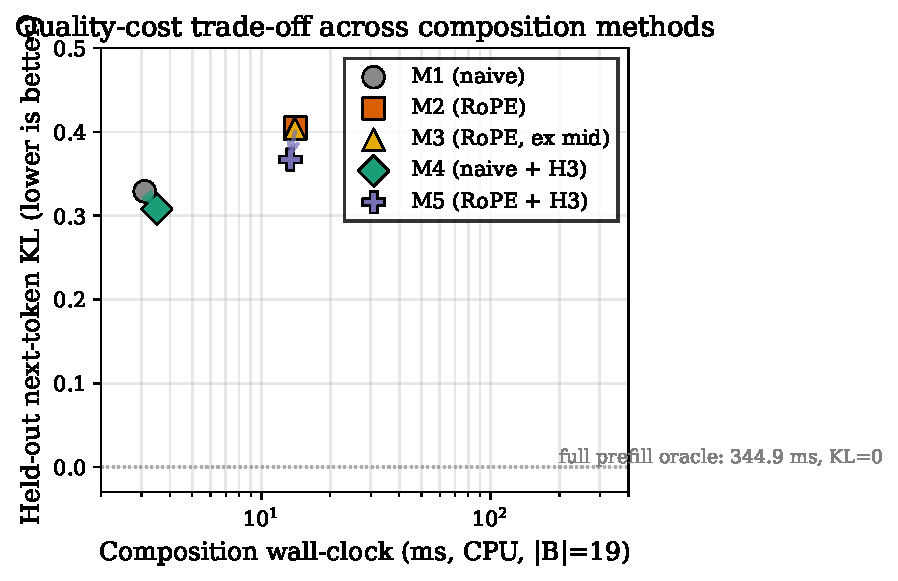
\includegraphics[width=\textwidth]{pareto.pdf}
\caption{Quality--cost trade-off across composition methods. Left: held-out next-token KL (Table~\ref{tab:holdout} aggregate), sorted with the best on top; dashed lines mark the M1 (grey) and M2 (red) baselines so the H3-augmented rows read directly as leftward improvements. Right: composition wall-clock in the same method order (Table~\ref{tab:cost}), with a dashed reference at the full-prefill cost (345~ms). Setup: Qwen-2.5-0.5B, CPU, $|B|=19$, $\mathrm{KV}_A, \mathrm{KV}_B$ already computed and in memory.}
\label{fig:pareto}
\end{figure}

\section{Discussion}

Our headline number is not the eye-catching $-35\%$ KL on the conflicting condition alone, but the more modest $-6.4\%$ (M4 vs M1) and $-9.4\%$ (M5 vs M2) held-out aggregate. These are the numbers that a linear map generalizes to unseen examples, at essentially zero cost, on a controlled benchmark whose baseline is trusted to $\approx 3\times10^{-7}$ KL.

Two qualitative findings we did not anticipate stand out:

\paragraph{Top-1 improvements can coexist with KL degradation.} On independent, referential, and cross-inferential conditions, M2 (RoPE-shift) improves top-1 while worsening KL relative to M1. This means the shift moves the argmax onto the oracle's argmax while shifting probability mass \emph{elsewhere} in the distribution. For open-ended generation this may not matter; for calibration-sensitive downstream use it might. Any composition method's evaluation must report both metrics.

\paragraph{RoPE-shift and H3 are complementary.} On the conflicting condition, M5 achieves the strongest individual reduction (0.353 $\to$ 0.228 held-out, top-1 $1.00$), suggesting that the two error sources (position and cross-context) can be attacked in the same pipeline without interference.

\section{Limitations}

We are explicit about what this study does \emph{not} yet show.

\begin{itemize}[leftmargin=*]
    \item \textbf{Model scale.} Qwen-2.5-0.5B only. Larger models may exhibit different layer-wise divergence patterns, and their baselines are typically more reliable on referential and reasoning queries; on the current model, the baseline itself fails cross-inferential arithmetic in some examples, muddying KL comparisons.
    \item \textbf{Model family.} Only Qwen tested; different RoPE bases, GQA structures, or attention patterns in Llama, Mistral, or Gemma may respond differently.
    \item \textbf{Realistic workloads.} 20 hand-crafted controlled examples. RAG, long-context QA, and multi-turn dialogue are unexplored.
    \item \textbf{Sample size and leakage.} $n=5$ per condition; example templates share entity and structural patterns. A larger benchmark with entity, length, and template variation is a near-term follow-up.
    \item \textbf{Corrector expressivity.} A single target layer ($l^\star=12$) and a linear map. Whether an MLP, an $A$-context-conditional corrector, or a multi-layer application yields larger gains is untested.
    \item \textbf{Composition depth.} Only two prefixes. Chains ($A + B + C + \ldots$) are unexplored.
\end{itemize}

None of these blockers is fatal to the direction; each is the subject of a concrete follow-up experiment in the project's public repository.

\section{Conclusion}

We separately analyzed two conceptual error sources of independent-prefill KV composition -- a position component fixable by RoPE-shift, and a cross-context representation component that is not -- and showed on a $20$-example controlled benchmark that a single $64\times64$ linear map on the mid-layer value cache reduces held-out downstream next-token KL by $6.4$--$9.4\%$ in aggregate and reduces KL on each of the four conditions. The corrector generalizes from 16 training to 4 held-out examples per fold within $3\times10^{-3}$ KL, and adds approximately $0.34$ ms and $0.0021\%$ of the FLOPs of one $B$-prefill. Scaling the benchmark, reproducing on larger and more diverse models, and testing more expressive correctors are the natural next steps.

\paragraph{Code and reproduction.} All code, data conditions, raw result logs, sanity checks, and cost measurements are released at \url{https://github.com/yunhyuk-mun/composable-kv} under an MIT license.

\bibliographystyle{plainnat}
\bibliography{references}

\appendix

\section{Pipeline sanity checks}\label{app:sanity}

We report four sanity checks against which every downstream number in this paper is measured. Numerical bounds are reported to make the noise floor of the composition pipeline explicit.

\begin{enumerate}[leftmargin=*]
    \item \textbf{Round-trip} (KL is preserved by cache injection). For every example $(A, B, Q)$ we tokenize once as $[A; B; Q]$ and compare next-token distribution of two routes: (i) $\mathrm{prefill}([A;B])$ followed by an incremental forward on $Q$ with the prefix cache; (ii) direct $\mathrm{prefill}([A;B;Q])$. Both routes must consume identical token ids to control for BPE boundary effects.
    Result: maximum KL across the 20 examples is $3.13\times10^{-7}$.
    \item \textbf{RoPE-shift(0)} is the identity map on $K$. Result: maximum $|K - R(0)K|$ over all 24 layers is $0.0$ (exact).
    \item \textbf{Determinism}: two independent prefill runs of the same input produce bitwise-identical $K$ and $V$. Result: exact.
    \item \textbf{Causal $A$-portion}: because the joint prefill is causal, tokens in $A$ cannot attend to $B$; their contribution to the joint cache should equal the $A$-alone cache. Result: maximum $|K^{(l)}_{\text{full}, :|A|} - K^{(l)}_A|$ is $1.53\times10^{-5}$, and similarly $5.25\times10^{-6}$ for $V$. This is at the expected float32 precision floor.
    \item \textbf{Tokenization boundary drift} (informational, not pass/fail). We compare the token id sequence produced by $\mathrm{tokenize}(A) + \mathrm{tokenize}(B) + \mathrm{tokenize}(Q)$ (used by the composition path) against the sequence produced by $\mathrm{tokenize}(A + \text{`` ''} + B + Q)$ (used by the ``from-scratch'' baseline path in \texttt{mve.py} and by \texttt{h3\_holdout.py}'s $p_{\text{full}}$). Result: 20/20 examples exhibit a boundary-length difference of $1$--$2$ tokens; where lengths coincidentally match, the interior token ids are identical. \emph{Consequence.} The absolute KL numbers in Tables~\ref{tab:main} and~\ref{tab:holdout} contain a small BPE-boundary artifact in addition to the composition error. Because every composition method is compared against the same baseline and shares the same drift, the \emph{relative} deltas ($\Delta$KL between methods) remain the intended measurement. A follow-up experiment enforcing identical token ids on both paths will refine the absolute magnitudes.
\end{enumerate}

Because the observed downstream method deltas (Table~\ref{tab:main}) are on the order of $10^{-2}$ KL, they are approximately $10^5$ times the round-trip noise floor, and their attribution to composition behavior (rather than injection artifacts) is safe. Check 5 above documents a small tokenization drift that affects absolute KL magnitudes but not the between-method deltas that this paper's claims are stated in.

\end{document}
